\documentclass[10pt]{article}
\textheight=9.25in \textwidth=7in \topmargin=-.75in
 \oddsidemargin=-0.25in
\evensidemargin=-0.25in
\usepackage{url}  % The bib file uses this
\usepackage{graphicx} %to import pictures
\usepackage{amsmath, amssymb}
\usepackage{theorem, multicol, color}
\usepackage{gfsartemisia-euler}

\setlength{\intextsep}{5mm} \setlength{\textfloatsep}{5mm}
\setlength{\floatsep}{5mm}
\setlength{\parindent}{0em} % new paragraphs are not indented
\setcounter{MaxMatrixCols}{20}
\usepackage{caption}
\captionsetup[figure]{font=small}


%%%%  SHORTCUT COMMANDS  %%%%
\newcommand{\ds}{\displaystyle}
\newcommand{\Z}{\mathbb{Z}}
\newcommand{\arc}{\rightarrow}
\newcommand{\R}{\mathbb{R}}
\newcommand{\N}{\mathbb{N}}
\newcommand{\Q}{\mathbb{Q}}
\renewcommand{\P}{\mathbb{P}}
\newcommand{\blank}{\underline{\hspace{0.33in}}}
\newcommand{\qand}{\quad and \quad}
\renewcommand{\stirling}[2]{\genfrac{\{}{\}}{0pt}{}{#1}{#2}}
\newcommand{\dydx}{\ds \frac{d y}{d x}}
\newcommand{\ddx}{\ds \frac{d}{d x}}
\newcommand{\dvdx}{\ds \frac{d v}{d x}} 

%%%%  footnote style %%%%

\renewcommand{\thefootnote}{\fnsymbol{footnote}}

\pagestyle{empty}

\begin{document}

\begin{flushright}
Chandler Justice - A02313187
\end{flushright}
\noindent \underline{\hspace{3in}}\\
\textbf{ST - Reinforcement Learning:} Homework \#2\\
\textbf{Due:}October 8, 2025 @ 23:59\\

\section{Part A: Conceptual Foundation}

\subsection{How DQN Extends Q-Learning}

Traditional Q-learning is done with a tabular representation of the state, where columns represent the state space, and the rows represent the action space\footnote{the decision to pick what is rows and what is columns is arbitrary}. At each cell of this table the value of the action value pair is provided. This gives us a function $Q(s,a)$, and as training time increases this table converges to an optimal solution $Q^*(s,a)$. As the environment increases in complexity, this tabular approach quickly becomes infeasible since the amount of memory required to hold the table explodes for any non-trivial environment. DQN solves this problem by using a \textit{deep} neural network\footnote{Deep means a neural network with hidden layers} to approximate $Q(s,a)$, we call this network the Q-network. 

\subsection{The Role of The Target Network}

We can converge a network to approximate this function by using the loss between a function denoted the target network and the reward obtained by the Q-network. The target function is updated less frequently which provides model stability and prevents undesired behavior such as oscillations in policy.\\

\subsection{The Replay Buffer}

Beyond these advancements, DQN also provides a \textit{replay buffer} which is used to revisit past experiences and reinforce the loss of that experience. While this might seem arbitrary at face value, the benefit of the replay buffer comes in reducing the local optima that can be reached in sequential experiences. In other words, a side effect of the replay buffer is its ability to push a model out of a local loss minima and towards the global loss minima.

\subsection{Approximation of the Bellman Equation}

In Q-learning, the Q-table is updated using the Bellman Equation

\[Q^*(s,a) = \mathbb{E}_{s' \sim \mathcal{E}} \left[r + \gamma \underset{a'}{\text{max}}Q^*(s', a')| s,a\right],\]

which says at $(s,a)$, our state-action pair, the optimal strategy is to select the action $a'$ which maximizes the expected value of $r + \gamma Q*(s',a')$. This would be prohibitively expensive to compute as stated previously. Instead, we can use a loss function

\[L_i (\theta_i) = \mathbb{E}_{s, a \sim p(\cdot)} \left[(y_i - Q(s,a;\theta_i))^2\right]\]

where $\theta$ is is the weights of the Q-network, $y_i$ is the value of the target network, and $Q$ is the value of the policy network. Using the gradient of this loss function, we are able to back propagate the network and eventually converge to an approximation of the value network\footnote{not quite $\blacksquare$, but it feels like a proof would be cool here.}.


\subsection{MDP (from HW1) versus Deep Q-Learning}

In homework 1, we trained a policy from a random actor, but the actor's policy was not iterated on. DQN is an \textit{online} algorithm meaning that the policy is changed during training. Additionally, the MDP implementation only updated the policy at the end of the episode, while DQN is updated more frequently. The MDP also relied on a tabular representation which is very computationally inefficient.

\section{Part B: DQN Implementation}

\begin{figure}[h!]
    \centering
    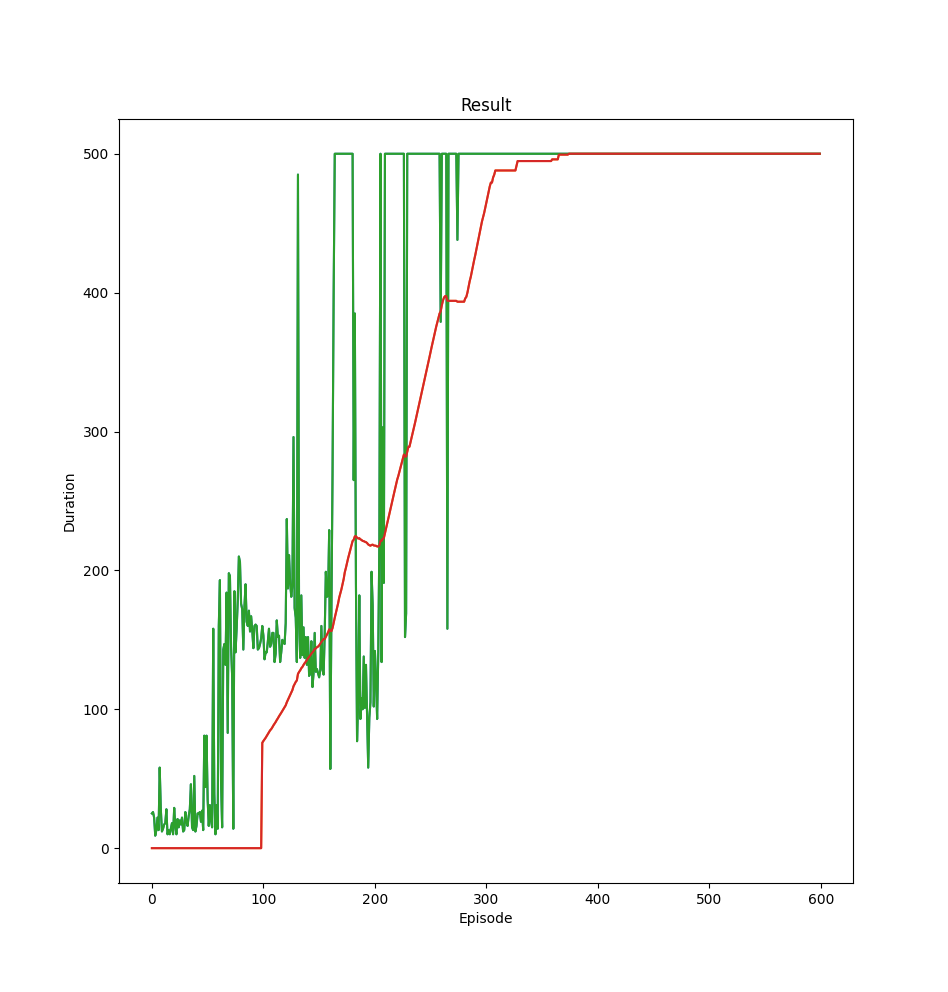
\includegraphics[scale=0.5]{cartpole_dqn_result.png}
    \caption{DQN Training on Gymnasium Cartpole Environment. Green is the reward at every episode, red is the average reward over 100 episodes}
\end{figure}

This is the implementation provided in the cartpole tutorial. The green line is the reward at every episode, and the red is the average across many episodes. The policy appears to converge at around 300 episodes.


\newpage

\section{Part C: Double DQN}

\begin{figure}[h!]
    \centering
    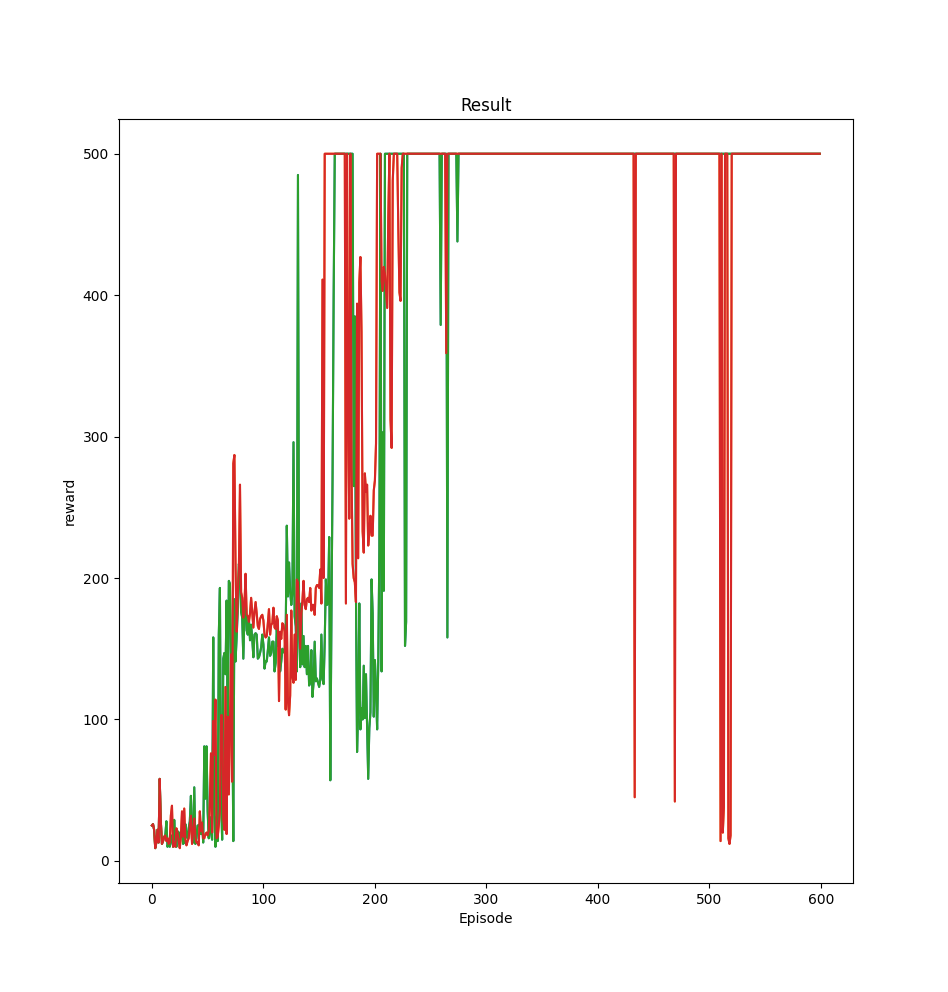
\includegraphics[scale=0.5]{dqn_green_ddqn_red_final_run.png}
    \caption{DQN and DDQN with default hyperparameters. DQN is green, DDQN is red.}
\end{figure}

We can see that DDQN in earlier episodes finds a better policy. Additionally, double DQN seems to act more stable. I believe the divergence seen towards the end of the run can be attributed to random sampling and lack of tuning around the hyperparameters.  

\newpage

\section{Part D: Double DQN Compared to DQN}

Double DQN tends to be more stable since in optimization it uses the target network to select actions, but uses the target network to evaluate the value of those actions. DQN tends to overestimate due to the max operator in its optimization. This leads to inflated values over time.\\

To test my conjecture of the dropoffs in reward seen in the previous section, I decreased epsilon decay so the agent would explore less. For DQN, this resulted in a much less stable policy which failed to converge in 600 iterations; however, this appears to result in a significantly improved convergence rate for DDQN. 

\begin{figure}[h!]
    \centering
    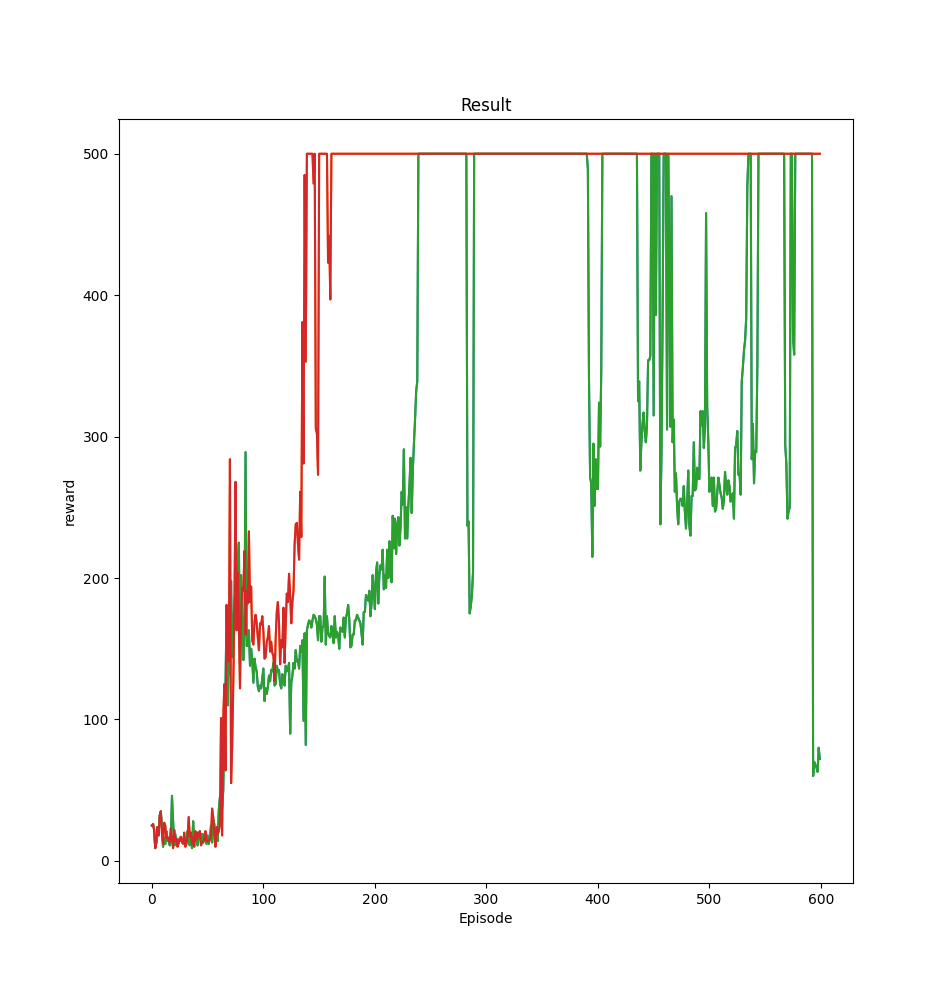
\includegraphics[scale=0.5]{dqn_green_ddqn_red_low_decay.png}
    \caption{DQN and DDQN with a faster epsilon decay. Green is DQN, red is DDQN.}
\end{figure}


\newpage

\section{Part E: Prioritized Experience Replay}

\begin{figure}[h!]
    \centering
    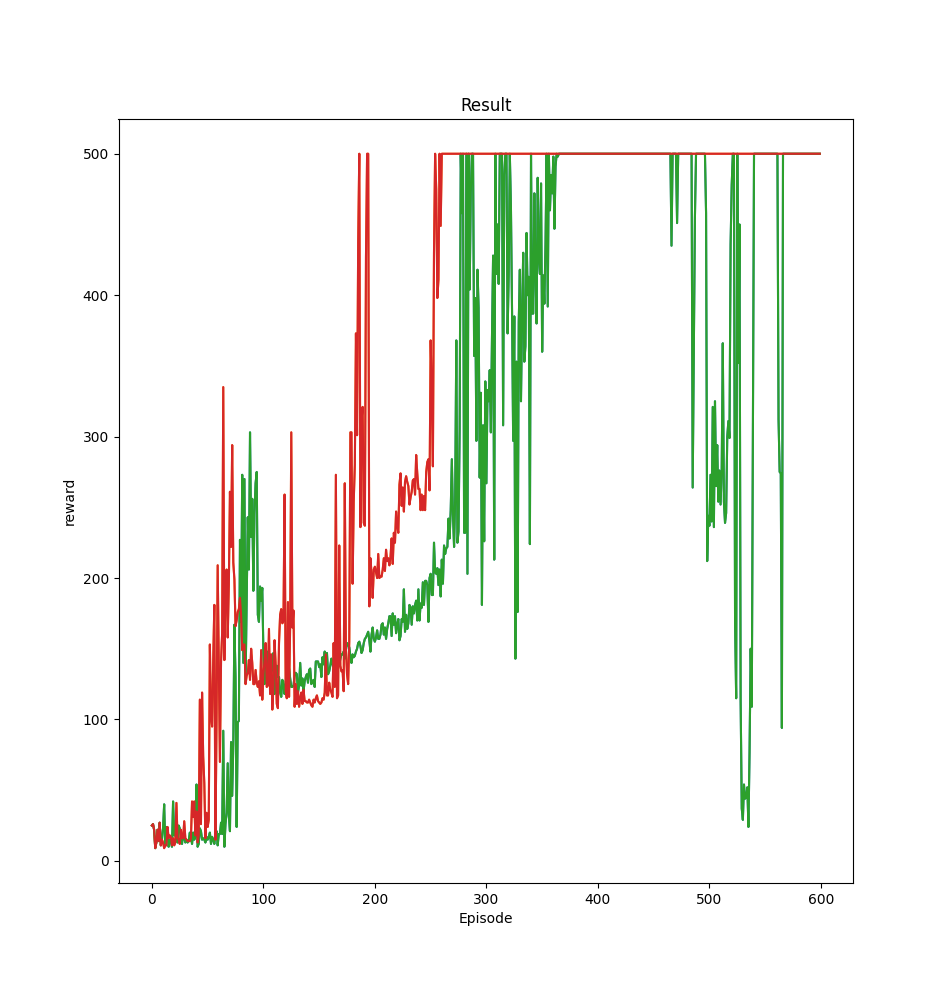
\includegraphics[scale=0.5]{per_ddqn_red_dqn_green.png}
    \caption{DQN and DDQN with prioritized experience replay. DQN is green, DDQN is red.}
\end{figure}

For DQN, performance appears to degrade when using PER. This could be due to the overestimation bias discussed in the previous part, with PER reinforcing bad behavior. DDQN appears to improve when using PER, resulting in convergence around 200 episodes versus $\approx$250 when using uniform sampling. 




\noindent \underline{\hspace{3in}}\\

\end{document}

